\documentclass[14pt]{extarticle}
\usepackage[
left=30mm,
top=20mm,
right=15mm,
bottom=20mm,
]{geometry}

\usepackage{graphicx}
\usepackage[utf8x]{inputenc}
\usepackage[russian]{babel}
\usepackage[T1]{fontenc}
\usepackage{float}
\usepackage{listings}
\usepackage{cite}
\usepackage{hyperref}
\usepackage{etoolbox}
\usepackage{indentfirst}
\usepackage[linesnumbered,boxed]{algorithm2e}
\sloppy

\graphicspath{{Figures//}}%путь к рисункам


\lstset{inputencoding=utf8x, extendedchars=false, keepspaces = true,
language=C++,
keywords={include, const, virtual, template, typename, class, private, public, operator, if, while, else, return, new, delete, int, float, bool, char},
sensitive=true,
%basicstyle=\small,
commentstyle=\scriptsize\rmfamily,
keywordstyle=\ttfamily\underbar,
identifierstyle=\ttfamily,
basewidth={0.5em,0.5em},
columns=fixed,
fontadjust=true,
breaklines=true,
literate={->}{{$\to$}}1
}

\makeatletter
\renewcommand{\@biblabel}[1]{#1.} % Заменяем библиографию с квадратных скобок на точку:
\makeatother
\gappto\captionsrussian{\renewcommand{\contentsname}{Оглавление}}
\renewcommand\baselinestretch{1.5}
\renewcommand{\lstlistingname}{Результат}

\begin{document}

\begin{titlepage}
\thispagestyle{empty}
\def\baselinestretch{1.0}
\begin{center}
	{САНКТ-ПЕТЕРБУРГСКИЙ ГОСУДАРСТВЕННЫЙ УНИВЕРСИТЕТ \\ \vskip 0.3em {\large Математико-механический факультет \\ \vskip 0.7em{\large Кафедра информатики \\}}}
    \vspace*{0.15\textheight}
    {\large Крень Мария}
    
    \vskip 2em
    {\huge Пользовательский уровень библиотеки неконсервативной сборки мусора для C++}
    
    \vskip 1em
    {\large Дипломная работа} \\
    \vskip 2em
    {\normalsize \raggedleft 
    Допущена к защите.\\
    Зав. кафедрой:\\
    д.ф.-м.н., Н.К.Косовский 
    \\[3em]
    Научный руководитель:\\
    к.ф.-м.н. Д.Ю.Булычев
    \\[3em]
    Рецензент:\\
    к.ф.-м.н. Д.В.Кознов\\
    \vspace*{0.08\textheight}
    {\centering Санкт-Петербург \\ 2014}
    }
\end{center}
\end{titlepage}
\begin{titlepage}
\thispagestyle{empty}
\def\baselinestretch{1.0}
\begin{center}
	{\large SAINT-PETERSBURG STATE UNIVERSITY \\ \vskip 0.3em {\large Mathematics and Mechanics Faculty \\ \vskip 0.7em{\large Informatics Chair \\}}}
    \vspace*{0.15\textheight}
    {\large Mariya Kren}
    
    \vskip 2em
    {\huge User Level of a Non-Conservative Garbage Collection Library for C++}
    
    \vskip 1em
    {\large Graduation Thesis} \\
    \vskip 2em
    {\normalsize \raggedleft 
    Admitted for defence.\\
    Head of the chair:\\
    professor N.K. Kosovsky
    \\[3em]
    Scientific supervisor:\\
    Dr. D.Yu. Boulytchev
    \\[3em]
    Reviewer:\\
    Dr. D.V.Koznov\\
    \vspace*{0.08\textheight}
    {\centering Saint-Petersburg \\ 2014}
    }
\end{center}
\end{titlepage}
\tableofcontents
\thispagestyle{empty} 
\section*{Введение}

Ручное управление памятью в языках, подобных C++, является источником большого количества трудно отслеживаемых ошибок, наличия которых можно было бы
избежать, сделав процесс управления памятью автоматическим. \textit{Сборка мусора} является одним из способов автоматического управления памятью, при
котором освобождение памяти выводится из-под контроля ПО на прикладном уровне. При автоматическом управлении программист не может явно влиять на распределение
объектов в памяти, у него есть лишь
косвенные способы сделать это с помощью использования тех или иных языковых конструкций. В идеальном случае, для рационального использования
памяти необходимо освобождать память, занимаемую объектами, которые более не будут использованы программой. Поскольку точно определить, что
объект не будет использован в дальнейшем, невозможно, на практике используют критерий доступности. \textit{Доступность} --- это консервативное
приближение используемости. \textit{Мусором}, в таком случае, называют объект, все пути доступа к которому уже разрушены, а память из-под него
ещё не освобождена. В некоторое, заранее определенное время, например, в простейшем случае, когда перестаёт хватать свободной памяти, выполнение
программы временно приостанавливается и запускается процесс \textit{сборки мусора}, который освобождает всю или ту, что возможно, память,
занятую мусором, после чего управление возвращается обратно программе. \textit{Сборщиком мусора} называется компонент, производящий \textit{сборку мусора}.

Процесс \textit{сборки мусора}, в простейшем случае, делят на три этапа:
\begin{enumerate}
\item \textit{Построение корневого множества}. На этом этапе строится множество объектов, которые считаются изначально доступными.
Такие объекты называются \textit{корнями} (англ. roots). Данное построение
аксиоматично, т.е. основывается на некотором наборе правил, согласно которым те или иные элементы считаются доступными. Данный этап является неотъемлемой
частью любого сборщика мусора.
\item \textit{Маркировка}. Начиная с множества, построенного на предыдущем этапе, происходит сканирование памяти, и все объекты, до которых возможно
добраться из построенного корневого множества, считаются доступными; оставшиеся объекты считаются мусором.
\item \textit{Освобождение}. Происходит сканирование кучи, в течение которого память из-под всех элементов, помеченных как мусор или не отмеченных как
доступные, освобождается.
\end{enumerate}

Есть несколько требований, которые должны быть выполнены для реализации сборки мусора:
\begin{enumerate}
\item Возможность построения корневого множества. Иными словами, необходимо иметь возможность идентифицировать все указатели в программном стеке, регистрах
и статической области памяти.
\item Должна присутствовать возможность определить все указатели из любого объекта на другие элементы кучи.
\end{enumerate}
В таких языках, как LISP или JAVA все условия соблюдаются, и в них успешно используется технология сборки мусора, в то время как, например,
в языке C не все условия выполняются. В языках, где не соблюдаются хотя бы одно из вышеперечисленных условий, возможна исключительна
\textit{консервативная сборка мусора}.
\textit{Консервативной} называется такая сборка мусора, при которой любой элемент данных, значение которого может быть истолковано, как указатель на
некоторый элемент кучи, считается  таковым. Консервативный подход к сборке мусора не позволяет собрать весь мусор, что может стать проблемой при обработке
большого количества данных. Неконсервативная сборка мусора лишена подобного недостатка и способна освободить всю память программы, более не
являющуюся доступной. \textit{Неконсервативным} или  \textit{точным сборком мусора} называется сборщик мусора, имеющий возможность точно распознать
все указатели в памяти. Иными словами, точный сборщик мусора --- это сборщик мусора, не использующий консервативный подход.

В C++ не соблюдаются требования, необходимые для сборки сборки мусора, реализовать точный сборщик мусора без ограничений
на использование некоторых примитивов языка не представляется возможным.
Более того, в C++ имеется ряд технических сложностей, затрудняющих реализацию точного сборщика мусора.
Тем не менее, в случае соблюдения программистом некоторых соглашений на програмный код,
точная сборка мусора становится возможной и в C++.

Целями работы является реализация основных примитивов библиотеки неконсервативной сборки мусора для C++,
обеспечение возможности совмещения ручного и автоматического управления памятью.
\newpage
\section{Постановка задачи}

Целью данной работы является создание пользовательского уровня для библиотеки неконсервативной сборки 
мусора для С++. Следующие основные подзадачи были выделены для её достижения:

\begin{itemize}
\item изучить и проанализировать существующие подходы к автоматизации управлением памятью 
для языка С++;

\item предложить и реализовать собственное решение на основе проведенного анализа;

\item продемонстрировать работоспособность реализованного сборщика мусора.
\end{itemize}

\newpage
\section{Обзор существующих библиотек}

В рамках исследования был проведен анализ основных существующих функциональных принтер-библиотек. Все выбранные библиотеки оказались комбинаторными, что естественно для функциональных языков.

% Так как работа проводилась в контексте функциональных языков, для анализа были выбраны комбинаторные библиотеки.
% Комбинаторы естественным образом возникают при наличии в языке функций высших порядков.

\subsection{Модельный язык L}
% \addcontentsline{toc}{section}{Модельный язык L}

В дальнейшем центральным примером, для которого мы будем разрабатывать принтеры, будет модельный язык L. Именно для этого языка будет реализован шаблонный принтер.

Язык L состоит из небольшого числа операторов:
\begin{enumerate}
	\item присваивание;
	\item цикл с предусловием;
	\item ветвление;
	\item последовательное выполнение;
	\item чтение с занесением в переменную;
	\item печать целочисленного выражения.
\end{enumerate}

Также в языке есть выражения. Выражения бывают трех типов:
\begin{enumerate}
	\item константа;
	\item переменная;
	\item бинарная операция.
\end{enumerate}

На рисунке~\ref{fig:lEx} приведен пример программы на языке L. В данном случае, это программа, которая считывает с консоли два числа, а потом возводит второе число в степень, равную первому.

\begin{figure}[h!]
	\centering
	% \inputminted{pascal}{codes/lEx.l}
	\lstinputlisting[language=llang]{codes/lEx.l}
	\caption{Быстрое возведение в степень на языке L}
	\label{fig:lEx}
\end{figure}

\subsection{Библиотека Хьюза}

Библиотека Джона Хьюза\cite{hughes} считается первой комбинаторной принтер-библиотекой. Она основана на алгоритме, предложенном Дереком Оппеном \cite{oppen}, и по сути является его реализацией в функциональном стиле на языке Haskell\footnote{http://haskell.org}. Также библиотека Хьюза, расширенная Саймоном Пейтоном Джонсом \cite{peytonJones}, является стандартной принтер-библиотекой для языка Haskell.

% рассказать об оптимальном

В данной библиотеке ключевым типом является “\lstinline[language=Haskell]{Doc}”. Он представляет документ, который потом может быть переведен в строковое представление.
Основные комбинаторы для составления документа:
% \inputminted{haskell}{Podkopaev/codes/hughesBasicOperators.hs}
\lstinputlisting[language=Haskell]{Podkopaev/codes/hughesBasicOperators.hs}

Так, с помощью функции “\lstinline[language=Haskell]{text}” по строке получается документ, оператор “\textbf{<>}” соединяет два документа горизонтально (см. рисунок~\ref{fig:hughesHorComp}), а оператор “\textbf{\$\$}” соединяет документы вертикально (см. рисунок~\ref{fig:hughesVertComp}).

\begin{figure}[ht]
	\begin{subfigure}[b]{0.45\linewidth}
		\centering
		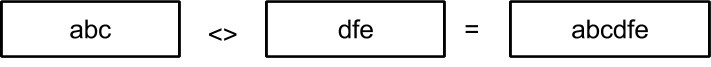
\includegraphics[width=\textwidth]{hughesHorComp}
		\caption{Комбинатор “\textbf{<>}”}
		\label{fig:hughesHorComp}
	\end{subfigure}
	\hspace{0.5cm}
	\begin{subfigure}[b]{0.45\linewidth}
		\centering
		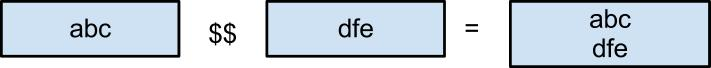
\includegraphics[width=\textwidth]{hughesVertComp}
		\caption{Комбинатор “\textbf{\$\$}”}
		\label{fig:hughesVertComp}
	\end{subfigure}

	\caption{Пример работы комбинаторов}
\end{figure}

Функция “\lstinline[language=Haskell]{nest}” добавляет к каждой строке документа заданное число ведущих пробелов. Функция “\lstinline[language=Haskell]{sep}” является ключевым комбинатором, который в этой библиотеке позволяет задавать плавающую раскладку документа. Она принимает как параметр список документов, а на выходе получается документ, который представляет из себя либо вертикальную склейку элементов списка, либо горизонтальную склейку (в этом случае если к документу из списка применялась функция “\lstinline[language=Haskell]{nest}”, то к этому документу не добавляются ведущие пробелы, то есть применение “\lstinline[language=Haskell]{nest}” попросту игнорируется), причем между документами вставляется пробельный символ. Вариант раскладки выбирается функцией “\lstinline[language=Haskell]{pretty}”:

% \inputminted{haskell}{Podkopaev/codes/hughesPretty.hs}
\lstinputlisting[language=Haskell]{Podkopaev/codes/hughesPretty.hs}

Кроме самого документа, функция “\lstinline[language=Haskell]{pretty}” также принимает два числа: максимальную длину и максимальную наполненность строки. Здесь наполненность строки значит длину текста без ведущих пробельных символов. В ходе работы этой функции и происходит выбор раскладки документа, полученного с помощью комбинатора “\lstinline[language=Haskell]{sep}”. Если горизонтальная раскладка удовлетворяет ограничениям на ширину строки, то она и выбирается. Иначе выбирается вертикальная раскладка.


% Возможно, стоит сделать после обзора всех библиотек

Рассмотрим пример описания принтера с помощью библиотеки Хьюза. Для этого используем учебный язык L. Часть принтера для языка L, отвечающая за представление операторов, показана на рисунке~\ref{fig:lHughesPrinter}.
В примере используется не описанный выше комбинатор “\lstinline[language=Haskell]{<+>}”, который определяется следующим образом:

\lstinputlisting[language=Haskell]{Podkopaev/codes/hughesAddComb.hs}

\begin{figure}[h!]
	% \inputminted{haskell}{Podkopaev/codes/lHughesPrinter.hs}
	\lstinputlisting[language=Haskell]{Podkopaev/codes/lHughesPrinter.hs}
	\caption{Принтер, написанный с помощью библиотеки Хьюза}
	\label{fig:lHughesPrinter}
\end{figure}

В данном случае принтер получился несложным, но абсолютно не наглядным. Поскольку в библиотеке нет механизмов, позволяющих явно варьировать раскладку документа в зависимости от раскладки его поддокументов, невозможно выразить пример с рисунка~\ref{fig:lGoodWriteEx}.
То есть, в случае многострочного выражения в операторе “\lstinline[language=llang]{write}”, напечатать закрывающую скобку на уровне самого оператора.

\begin{figure}[h!]
	% \inputminted{pascal}{Podkopaev/codes/lGoodWriteEx.l}
	\lstinputlisting[language=llang]{Podkopaev/codes/lGoodWriteEx.l}
	\caption{Желательный пример печати конструкции “\lstinline[language=llang]{write}”}
	\label{fig:lGoodWriteEx}
\end{figure}

С помощью реализации принтера с рисунка~\ref{fig:lHughesPrinter}, в данном случае для оператора “\lstinline[language=llang]{write}” получится немного не то (см. рисунок~\ref{fig:lCurWriteEx}).
\begin{figure}[h!]
	% \inputminted{pascal}{Podkopaev/codes/lCurWriteEx.l}
	\lstinputlisting[language=llang]{Podkopaev/codes/lCurWriteEx.l}
	\caption{Результат для изначального принтера конструкции “\lstinline[language=llang]{write}”}
	\label{fig:lCurWriteEx}
\end{figure}

Если попробовать поменять функцию “\lstinline[language=Haskell]{docFromOperation}” для конструкции “\lstinline[language=llang]{write}” (см. рис. \ref{fig:lHughesWriteChange}),
то для многострочного выражения все получится правильно, но в случае однострочного --- появится лишний пробел перед закрывающей скобкой (см. рис. \ref{fig:lBadWriteEx})).

\begin{figure}[h!]
	% \inputminted{haskell}{Podkopaev/codes/lHughesWriteChange.hs}
	\lstinputlisting[language=Haskell]{Podkopaev/codes/lHughesWriteChange.hs}
	\caption{Измененный принтер конструкции “\lstinline[language=llang]{write}”}
	\label{fig:lHughesWriteChange}
\end{figure}

\begin{figure}[h!]
	% \inputminted{pascal}{Podkopaev/codes/lBadWriteEx.l}
	\lstinputlisting[language=llang]{Podkopaev/codes/lBadWriteEx.l}
	\caption{Результат для измененого принтера конструкции “\lstinline[language=llang]{write}”}
	\label{fig:lBadWriteEx}
\end{figure}
\newpage

\subsection{Принтер-комбинаторная библиотека Вадлера}

В \cite{wadler} Филипп Вадлер описал свою комбинаторную бибилиотеку для форматированного вывода на языке Haskell. Она является модификацией библиотеки Хьюза, описанной в предыдущем разделе. Код библиотеки сократился с $\approx$ 110 строк до $\approx$ 80 строк, и, по исследованию Вадлера, на 30\% увеличилась скорость вычисления раскладки документа.

Рассмотрим основые комбинаторы этой библиотеки:
% \inputminted{haskell}{codes/wadlerBasicOperations.hs}
\lstinputlisting[language=Haskell]{codes/wadlerBasicOperations.hs}

Вадлер решил отказаться от двух разных способов соединения документов, оставив лишь горизонтальную склейку. Но для того, чтобы можно было выражать не только однострочные документы, в библиотеке Вадлера появилась функция “\lstinline[language=Haskell]{line}”. Она создает документ, который может быть переведен в символ новой строки или в пробел.
Функция “\lstinline[language=Haskell]{group}” имеет то же назначение, что и оператор “\lstinline[language=Haskell]{sep}” в библиотеке Хьюза, но работает не со списком документов, а с одним документом, и по сути предоставляет альтернативы для алгоритма перевода документа в “\lstinline[language=Haskell]{String}”: в документе, на который подействовал “\lstinline[language=Haskell]{group}”, либо все вхождения “\lstinline[language=Haskell]{line}” заменяются на пробел, либо остаются переводами строки (если они не являются частью вложенных “\lstinline[language=Haskell]{group}”-документов).

В таком виде библиотека потеряла в выразительности, что признается в статье Вадлера. Но кроме потери выразительности, есть еще один серьезный недостаток, возникающий из-за оператора “\lstinline[language=Haskell]{group}”. То, что любой документ им может быть преобразован в однострочный, делает библиотеку неприменимой в некоторых ситуациях. 

Рассмотрим следующий пример. Пусть нам надо написать принтер для языка Python\footnote{http://python.org}. Для конструкции последовательных операторов принтер изображен на рисунке~\ref{fig:pythonPrinter}.
По-другому его написать нельзя --- мы хотим, чтобы последовательные операторы печатались на новых строках. Но если такая конструкция попадет внутрь “\lstinline[language=Haskell]{group}”-документа, то последовательные строчки могут склеиться пробелом, что сделает код некорректным, так как в Python несколько операторов на одной строке должны разделяться символом “;”.

\begin{figure}[h!]
	% \inputminted{haskell}{codes/pythonPrinter.hs}
	\lstinputlisting[language=Haskell]{codes/pythonPrinter.hs}
	\caption{Принтер для последовательных операторов в Python}
	\label{fig:pythonPrinter}
\end{figure}

Так корректный код (см. рисунок~\ref{fig:pythonCode}) может превратиться в некорректный (см. рисунок~\ref{fig:pythonCodeBad}).
\begin{figure}[h!]
	\centering
	\null\hfill
	\subfloat[]{
		\centering
		\lstinputlisting[language=Python]{codes/pythonCode.py}
		\label{fig:pythonCode}	
	}
	\null\hfill
	\subfloat[]{
		\centering
		\lstinputlisting[language=Python]{codes/pythonCodeBad.py}
		\label{fig:pythonCodeBad}
	}
	\hfill
	\null
	\caption{Пример работы принтера для языка Python}
\end{figure}

\newpage

\subsection{Библиотека Азеро и Свиерстры}

Библиотека Азеро и Свиерстры\footnote{
В данном тексте, с целью не усложнять восприятие, изменены обозначения комбинаторов библиотеки Свиерстры на обозначения, подобные тем, что были уже рассмотрены в библиотеке Хьюза. Семантика комбинаторов описана без изменений, согласно оригинальной статье и соответствующей библиотеке.
}, описанная в \cite{swierstra}, отличается от предыдущих библиотек тем, что дает возможность явным образом задать несколько несвязанных вариантов раскладки документа. В этой библиотеке есть комбинатор “\lstinline[language=Haskell]{<|>}”:

% \inputminted{haskell}{Podkopaev/codes/chooseSw.hs}
\lstinputlisting[language=Haskell]{Podkopaev/codes/chooseSw.hs}

Этот комбинатор берет два документа и создает новый, который при раскладке может стать первым или вторым, в зависимости от того, какой из документов раскладывается оптимальней. \textit{Оптимальной} раскладкой для документа считается раскладка, удовлетворяющая ограничению на ширину документа и имеющая минимальную высоту.

Наличие комбинатора “\lstinline[language=Haskell]{<|>}” сразу же решает проблему со скобкой, которая была поднята в обзоре библиотеки Хьюза (см. рис.~\ref{fig:bracketSwierstra}).\footnote{
	В примере используется функция “\lstinline[language=Haskell]{element_h1}”. Эта функция выбирает из вариантов раскладки документа те, которые имеют высоту 1.
}

\begin{figure}[h!]
	% \inputminted{haskell}{Podkopaev/codes/bracketSwierstra.hs}
	\lstinputlisting[language=Haskell]{Podkopaev/codes/bracketSwierstra.hs}
	\caption{Принтер конструкции “\lstinline{write}”, удовлетворяющий примеру с рис.~\ref{fig:lGoodWriteEx}}
	\label{fig:bracketSwierstra}
\end{figure}

% Данная вариативность достигается за счет особого представления документа. В данной библиотеке он представляется как ленивый список раскладок, причем список отсортирован в порядке возрастания количества строк раскладки.

Библиотека Азеро и Свиерстры обладает самым богатым набором комбинаторов и, благодаря оператору “\lstinline[language=Haskell]{<|>}”, позволяет выразить практически любые принтеры. Но, также как остальные рассмотренные библиотеки, не дает механизмов для простого и наглядного задания принтеров.
\newpage
\section{Используемые особенности языка С++}

Реализация сборки мусора в виде внешней библиотеки существенно опирается 
на некоторые особенности как языка С++, так и его компиляторов и среды поддержки времени 
исполнения. К таковым особенностям относятся:

\begin{enumerate}
\item функция \lstinline{typeid} и возможность идентификации типа во время исполнения (runtime type identification, RTTI);
\item инициализация по размещению (placement new);
\item шаблоны, в том числе шаблоны с переменным числом аргументов (templates, variadic templates);
\item конструкторы, деструкторы и порядок их вызова.
\end{enumerate}

Далее рассмотрим вышеперечисленные особенности подробнее.

\subsection{Функция \lstinline{typeid} и идентификация типа\\
во время исполнения} 

Идентификация типа во время исполнения позволяет получить метаинформацию о типе объекта во время работы программы. 
В сборщике мусора эта метаинформация используется для установления связи между объектом и метаинформацией сборщика
мусора, соответствующей этому типу. Для того, чтобы это стало возможно, поддержка RTTI должна быть включена 
соответствующими опциями компилятора.

На пользовательском уровне возможности RTTI представлены функцией \lstinline{typeid}\footnote{\url{http://www.c-cpp.ru/books/identifikaciya-tipa-vo-vremya-ispolneniya-rtti}},
которая получает указатель на объект и возвращает ссылку на объект типа \lstinline{typeinfo}. Данный тип
содержит информацию о типе объекта, в частности, имя этого типа, которое и используется в сборщике мусора.

\subsection{Инициализация по размещению, шаблоны,\\
шаблоны с произвольным числом аргументов} 

Инициализация по размещению и шаблоны с произвольным числом аргументов в реализации сборщика мусора используются 
совместно для того, чтобы выразить примитив выделения памяти. Основная задача, которая при этом возникает 
кроме собственно выделения~--- определение типа объекта, занимающего данную область памяти, и её аннотирование
соответствующей метаинформацией. 

Отследить момент выделения памяти можно было бы путем перегрузки глобального оператора \lstinline{new}; однако
в этом случае было бы трудно узнать, каков тип объекта, для которого выделяется память. Использование же
инициализации по размещению, шаблонов и шаблонов с произвольным числом аргументов позволяет инкапсулировать
всю нужную функциональность в одной функции, которая отведет память, вызовет конструктор, передав
ему нужное количество аргументов, и кроме того выполнит все остальные необходимые действия.

 \subsection{Конструкторы, деструкторы и порядок их вызова} 

Важным фактом является то, что в С++ момент создания/удаления объекта можно отследить с помощью 
конструктора/деструктора\footnote{\url{http://www.developerfusion.com/article/133063/constructors-in-c11/}}. 
В сборщике мусора это используется для того, чтобы, во-первых, построить метаинформацию для данного типа (каждый
``умный указатель'' при создании регистрирует себя в некоторой структуре данных) и, во-вторых, чтобы регистрировать
корневые указатели во внешнем пуле корней.

\newpage
\section {Пользовательский уровень библиотеки\\
сборки мусора}

С точки зрения пользователя библиотека сборки мусора представлена одним шаблонным классом
``умного указателя'' 

\begin{lstlisting}
    template <class T> class gc_ptr {
       ...
    }
\end{lstlisting}

и одной шаблонной функцией выделения памяти

\begin{lstlisting}
    template <class T, typename ... Types> T* gc_new (
    Types ... types, size_t count = 1
    ) {
       ...
    }
\end{lstlisting}

которые становятся доступными после подключения одного заголовочного файла:

\begin{lstlisting}
    # include <libgc/libgc.h>
\end{lstlisting}

Исполняемый код библиотеки содержится в модулях, которые могут быть как собраны статически вместе
с приложением, так и подгружены динамически.

Любая программа, которая в качестве примитива выделения памяти использует \lstinline{gc_new}, в качестве
указателей --- \lstinline{gc_ptr}, и не содержит явного освобождения памяти с помощью \lstinline{delete}, будет
работать с использованием сборки мусора.

Семантика описанных примитивов с точки зрения сборки мусора будет описана в следующем разделе; пока же
мы обсудим их интерфейс с точки зрения пользователя.

\subsection{Интерфейс \lstinline{gc_ptr}}

Класс \lstinline{gc_ptr} инкапсулирует всю функциональность указателя, которая безопасна с точки зрения
сборки мусора. Данный класс реализует следующие операторы:

\begin{enumerate}
\item \lstinline{T& operator*() const}~--- разыменование;
\item \lstinline{T* operator->() const, operator T* () const}~--- доступ к указателю;
\item \lstinline{T& operator[](size_t index)}~--- доступ к элементам массива;
\item \lstinline{bool operator== (const gc_ptr <T> &a), bool operator== (const T* a)}~--- проверки на равенство;
\item \lstinline{bool operator!= (const gc_ptr <T> &a), bool operator!= (const T* a)}~--- проверки на неравенство;
\item \lstinline{gc_ptr& operator = (const gc_ptr <T> &a), gc_ptr& operator = (T* a)}~--- присваивание.
\end{enumerate}

Кроме того, у данного класса два конструктора: \lstinline{gc_ptr (T* p)} и \lstinline{gc_ptr (const gc_ptr <T> &p)}. 

\subsection{Функция выделения памяти \lstinline{gc_new}}

В языке С++ существует пять различных вариантов выделения памяти с помощью оператора \lstinline{new}. 
Этот оператор пытается выделить достаточно памяти в куче для размещения новых данных и, в случае успеха, возвращает 
адрес выделенного участка. После выделения памяти вызывается конструктор создаваемого объекта. Однако, если оператор
\lstinline{new} не может выделить память в куче, то возбуждается исключение типа \lstinline{std::bad_alloc}. 

Функция \lstinline{gc_new} позволяет выразить все ситуации, в которых может быть употреблён оператор \lstinline{new}.
Ниже мы приведем примеры использования \lstinline{gc_new} в каждой из них.

\begin {enumerate}
\item \lstinline{gc_new<type> ()}~--- выделение памяти под значение атомарного типа (\lstinline{int}, \lstinline{float} и т.д.); 
\item \lstinline{gc_new<C> ()}~--- выделение памяти под одиночный экземпляр объект класса \lstinline{C} с вызовом конструктора по
умолчанию;
\item \lstinline{gc_new <type> (len)}~--- выделение памяти под массив длины \lstinline{len} из элементов атомарного типа \lstinline{type};
\item \lstinline{gc_new <C> (len)}~--- выделение памяти под массив длины \lstinline{len} из экземпляров класса \lstinline{C}, для каждого из
которых вызывается конструктор по умолчанию;
\item \lstinline{gc_new <C, T1, T2, ..> (a1, a2, ..)}~--- выделение памяти под экземпляр объекта класса \lstinline{C} с вызовом
конструктора с парамерами \lstinline{a1, a2, ..}, имеющими типы \lstinline{T1, T2, ..} соответственно.
\end {enumerate}

Таким образом примитив выделения памяти в языке С++ для объектов различных типов можно заменить вызовом функции \lstinline{gc_new} 
соответствующего вида.

\subsection{Пример использования пользовательских\\
примитивов}

В качестве примера использования пользовательских примитивов библиотеки сборки мусора приведем 
реализацию класса строк:

\begin{lstlisting}
    class GCString {
      private:
        gc_ptr<char> pData; 	
        int length;	 
        GCString (gc_ptr<char> p, int l) : pData (p), length (l) {};     
      public:
        GCString () : length (0), pData (NULL) {};
        GCString (const char *cString);
        virtual ~GCString () {};
        GCString (const GCString &s);
        GCString operator= (const GCString &s);
        GCString operator= (const char *cString);
        char operator[] (int i) {return pData [i];};
        GCString operator+  (const GCString &s);
        GCString operator+  (const char *cString);
        GCString operator+= (GCString& s);
      };

      GCString::GCString (const char *cString) {
        length = strlen (cString);
        pData  = gc_new<char> (length+1);
        strcpy ((char *) pData, cString);
      }

      GCString::GCString (const GCString &s) : 
        length (s.length), pData (s.pData) {}

      GCString GCString::operator= (const GCString &s) {
        length = s.length;
        pData  = s.pData;
        return *this;
      }

      GCString GCString::operator= (const char *cString) {
        return *this = GCString (cString);
      }

      GCString GCString::operator+ (const GCString &s) {
        gc_ptr<char> p = gc_new<char> (length + s.length + 1);
        strcpy (p, (char*) this->pData);
        strcat (p, (char*) s.pData);
        return GCString (p, length + s.length);
      }

      GCString GCString::operator+ (const char *cString) {
        return *this + GCString (cString);
      }

      GCString GCString::operator+= (GCString &s) {
        return *this = *this + s;
      }
\end{lstlisting}

\newpage
\section{Семантика примитивов\\
пользовательского уровня\\
с точки зрения сборки мусора}

Одним из самых популярных алгоритмов сборки мусора является  алгоритм ``\emph{пометки и 
освобождения}'' (mark-and-sweep). Его популярность обусловлена простотой и тем, что 
данный алгоритм накладывает минимальные ограничения на организацию поддержки времени
исполнения и требует минимальной поддержки со стороны компилятора. 

Задачи, решаемые в процессе организации сборщика мусора такого типа, показаны на Рис.~1.

\begin{figure}[h!]
	\centering
	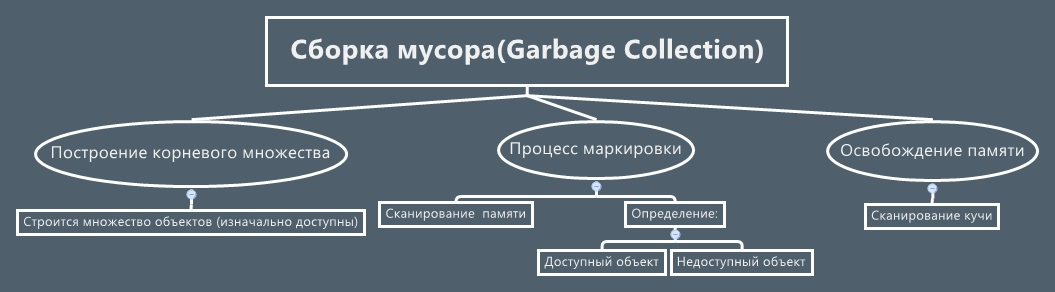
\includegraphics[width=500pt]{picture1.jpg}
	\caption{Три основных этапа сборки мусора}
	\centering
\end{figure}

Алгоритм ``пометки и освобождения'' состоит из двух фаз, которые запускаются последовательно
одна за другой:

\begin{itemize}
\item Фаза пометки. Начиная с некоторого аксиоматически заданного множества указателей, называемого
\emph{корневым множеством}, происходит полный обход всех достижимых объектов. Каждый достижимый
объект помечается как живой.
\item Фаза освобождения. Происходит полный обход кучи, во время которого освобождается память
из-подо всех непомеченных объектов; при этом пометка с помеченых объектов снимается.
\end{itemize}

Для реализации сборки мусора с помощью алгоритма ``пометки и освобождения'' должны быть решены
следующие задачи:

\begin{enumerate}
\item Идентификация корневого множества. Корневое множество~--- это множество указателей на
объекты, которые считаются изначально доступными для программы. Такие указатели хранятся в
стеке, регистрах и статической области памяти. В задачу идентификации корневого множества 
входит распознавание указателей в кучу на отведенные там объекты среди всех таких значений.

\item Определение всех ссылок из данного объекта на другие объекты в куче, что необходимо для
обхода всех достижимых объектов в фазе пометки.

\item Обеспечение возможности пометки объектов в куче и обхода всей кучи с освобождением 
непомеченных объектов.
\end{enumerate}

Последняя задача относится к реализации кучи; её решение изложено в~\cite{realisation}. Ниже 
мы опишем, как с помощью пользовательских примитивов, введенных в предыдущем разделе,
нами решаются две первые задачи.

\subsection{Поддержка корневого множества}

Идентификация корневого множества указателей (то есть указателей, хранящихся на стеке, в регистрах и статической
области памяти) без помощи со стороны компилятора является серьезной проблемой~\cite{roots}. При ``библиотечном''
подходе к сборке мусора рассчитывать на поддержку со стороны компилятора не приходится, поэтому в момент
начала сборки мусора идентифицировать корневые указатели уже невозможно. Поэтому корневое множество
поддерживается по мере работы программы. В него добавляются все \lstinline{gc_ptr}, экземпляры которых
не созданы с помощью \lstinline{gc_new}. Для этого в функции \lstinline{gc_new} выставляется флаг,
который проверяется в конструкторе \lstinline{gc_ptr}; в этом же конструкторе происходит добавление
указателя на объект \lstinline{gc_ptr} в пул корней, если это необходимо. Удаление же корневого
указателя происходит при вызове его деструктора. Так как удалять нужно только корневые указатели, а деструкторы
вызываются для всех, в \lstinline{gc_ptr} хранится признак того, что это корень. Поскольку деструкторы 
вызывается по отношению к конструкторам в обратном порядке (для автоматических объектов), пул корней можно 
реализовать в виде стека в отдельной области памяти вне кучи. 

\subsection{Построение метаинформации}

Представление метаинформации для сборки мусора, использованное нами, близко к тому, что описано
в~\cite{meta}. Метаинформация для типа представляет собой вектор смещений объектов \lstinline{gc_ptr} 
относительно начала экземпляра этого типа. Функция \lstinline{gc_new}, используемая для создания объектов, 
осуществляет поиск метаинформации по имени типа, полученному с помощью функции \lstinline{typeid}. 
Если этот поиск неуспешен (и, следовательно, для данного типа еще не была построена метаинформация), 
то создается новый объект, хранящий метаинформацию, и ассоциируется с именем этого типа. Для построения
метаинформации используются вызовы конструкторов \lstinline{gc_ptr}, с помощью которых можно
посчитать разность между адресом начала объекта и адресом, по которому ``внутри'' него расположен данный
\lstinline{gc_ptr}. 

После получения метаинформации функция \lstinline{gc_new} размещает указатель на неё перед данными 
создаваемого объекта. Это даёт возможность по указателю на живой объект узнать все указатели
из него на другие живые объекты, то есть реализовать стадию маркировки.

\newpage
\section{Заключение}

В результате выполнения данной дипломной работы были достигнуты следующие результаты:

\begin{enumerate}
\item изучены различные способы автоматизации управления памятью для языка C++ на 
основе использования ``умных указателей'';

\item разработан интерфейс библиотеки, позволяющей реализовать неконсервативную сборку мусора
при выполнении определенных соглашений на вид использующей её программы.

\item данное решение было использовано в рамках проекта по разработке библиотеки неконсервативной 
сборки мусора для языка С++;

\item полученная библиотека была протестирована на ряде примеров.
\end{enumerate}

%\newpage
\bibliographystyle{plainnat}
\addcontentsline{toc}{section}{Список литературы}
\begin{thebibliography}{}

\bibitem{GCBook} 
Richard Jones, Rafael Lins. Garbage Collection: Algorithms for Automatic Dynamic Memory Management. John Wiley \& Sons, 2001.

\bibitem{roots}
Д.А. Березун. Построение корневого множества указателей для сборки мусора // Труды лаборатории языковых инструментов JetBrains, 
выпуск 1. Санкт-Петербург, 2013.

\bibitem{meta}
М.В. Крень. Представление данных для сборки мусора // Труды лаборатории языковых инструментов JetBrains, выпуск 1. Санкт-Петербург, 2013.


\bibitem{realisation}
Д.А. Березун. Реализация основных примитивов библиотеки неконсервативной сборки мусора для С++. Дипломная работа, СПбГУ, 2014.


\bibitem{standart}
Bjarne Stroustrup. C++11 --- the new ISO C++ standard // \url{http://www.stroustrup.com/C++11FAQ.html}


\end{thebibliography}

%\newpage
%\appendix

\section*{Приложение}
\label{appendix}
\subsection*{Псевдокод алгоритма синтаксического анализа графов}

Пусть $(C_S, C_U, i, l)$ --- текущий дескриптор, где $C_S$ --- состояние рекурсивного автомата, представляющего грамматику, $C_U$ --- вершина GSS, $i$ --- вершина входного графа, $l$ --- длина разобранной части строки. Для получения имени нетерминала грамматики, соответствующего состоянию автомата используется функция $\Delta : Q \rightarrow N$. 

Во время работы алгоритма поддерживаются следующие множества: $R$ --- глобальная очередь дескрипторов, $U$ --- множество созданных ранее дескрипторов, $P$ --- множество, хранящее информацию о вызовах функции \textbf{pop}.

\begin{algorithmic}
\Function{add}{$S, u, i, l$}
	\If{($(S, u, i, l) \notin U$)}
		\State $U.add(S, u, i, l)$
		\State $R.enqueue(S, u, i, l)$
	\EndIf
\EndFunction
\end{algorithmic}

\begin{algorithmic}
\Function{create}{$S_{call}, S_{next}, u, i, l$}
	\State $A \gets \Delta(S_{call})$
	\If{($\exists$ GSS node labeled $(A, i)$)}  
		\State $v \gets$ GSS node labeled $(A, i)$
		\If{(there is no GSS edge from $v$ to $u$ labeled ($S_{next}, l$))}
			\State add GSS edge from $v$ to $u$ labeled ($S_{next}, l$)
			\For{($(v, j, m) \in P$)}
				\If{($S_{next}$ is a final state)}
					\State \Call{pop}{$u, j, (l + m)$}
				\EndIf
				\State \Call{add}{$S_{next}, u, j, (l + m)$}
			\EndFor
		\EndIf
	\Else
		\State $v \gets$ \textbf{new} GSS node labeled $(A, i)$
		\State create GSS edge from $v$ to $u$ labeled ($S_{next}, l$)
		\State \Call{add}{$S_{call}, v, i, 0$}
	\EndIf
\EndFunction
\end{algorithmic}

\begin{algorithmic}   
\Function{pop}{$u,i,l$}
	\If{($(u,i,l) \notin P$)}  
		\State $P.add(u,i,l)$
		\ForAll{GSS edges $(u,S,m,v)$}
			\If{($S$ is a final state)}
				\State \Call{pop}{$v, i, (l + m)$}
			\EndIf
			\State \Call{add}{$S, v, i, (l + m)$}
		\EndFor
	\EndIf
\EndFunction
\end{algorithmic}

\begin{algorithmic}
\Function{parse}{RA, input}
	\State $GSSroot\gets new GSSnode(RA.StartState, input.StartState) $
	\State $R.enqueue(RA.StartState, GSSroot, input.StartState, 0)$
	\While{$R \neq \varnothing $}
		\State{$(C_{S},C_{U},i,l) \gets R.dequeue()$}
	
		\If{ ($l = 0 $) and ($C_{S}$ is a final state)}
			\State \Call{pop}{$C_{U},i,0$}
		\EndIf
	
		\For{\textbf{each} $transition (C_{S},label,S_{next})$}
			\Switch{$label$}
			\Case{$Terminal(x)$}
				\For{\textbf{each} (input[i] $\xrightarrow[]{x}$ input[k])}
					\If{($S_{next}$ is a final state)}
						\State \Call{pop}{$C_U, k, (l + 1)$}
					\EndIf
					\If{$S_{next}$ have multiple ingoing transitions}
						\State \Call{add}{$S_{next}, C_{U}, k, (l + 1)$}
					\Else
						\State $R.enqueue(S_{next}, C_{U}, k, (l + 1))$
					\EndIf
				\EndFor
			\EndCase
			
			\Case{$Nonterminal(S_{call})$}
				\State \Call{create}{$S_{call}, S_{next}, C_{U}, i, l$}
			\EndCase
			\EndSwitch
		\EndFor
	\EndWhile
	\State $result \gets \emptyset$
	\For{\textbf{each} $(u, i, l) \in P$ where $u = GSSroot$, $i = input.FinalState$}
		\State $result.add(l)$
	\EndFor
	\If{$result \neq \emptyset$}
		\ return $result$
	\Else
		\ report failure
	\EndIf
\EndFunction
\end{algorithmic}


% \bibliographystyle{ugost2008ls}
% \bibliography{diploma.bib}

\end{document}
